\section{System Model}
\label{sec:system}

\subsection{Network and traffic}

We consider a single basic service set: one access point and $N = 16$ stations
on a 20\,MHz 802.11ax channel, with a beacon interval of
$T_{\mathrm{BI}} = 102.4$\,ms. All traffic is uplink.

Stations belong to four device classes, four each, representing mixed traffic:
a low-rate IoT sensor, a video camera, a voice assistant and a video streamer,
offering $0.058$, $2.037$, $0.030$ and $3.400$\,Mb/s respectively for
$22.1$\,Mb/s in aggregate. The access point acts once every $\Delta = 20$
beacon intervals, or $2.048$\,s: $42$ decisions per episode.

\subsection{Target Wake Time}

A TWT schedule partitions the beacon interval into $K$ service periods of
durations $\{w_1, \dots, w_K\}$. Each station is assigned to one group, and
group $k$ is awake from $\sum_{j<k} w_j$ to $\sum_{j \le k} w_j$ in every
beacon interval and sleeps outside it, so staggering trades contention against
window length. The catalogue holds $20$ schedules spanning one to four service
periods and $20$--$90$\,ms of wake time, with $19$ rules mapping the $16$
stations to groups. One-group schedules make several rules coincide, so the
$760$ encoded actions realise fewer distinct configurations.

\begin{figure}[t]
  \centering
  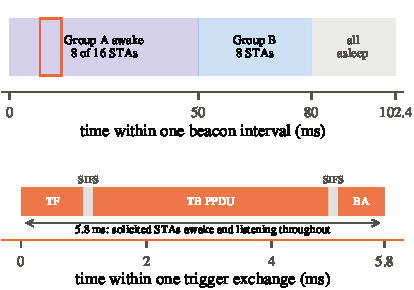
\includegraphics[width=\columnwidth]{figures/fig_system.pdf}
  \caption{\emph{Top:} one beacon interval under a two-group TWT schedule.
  \emph{Bottom:} a trigger exchange on its own scale. A solicited station is
  awake for the whole exchange---receiving, then transmitting its own
  reply---and the scheduler reserves the $5.8$\,ms worst case before admitting
  one, which is what makes uplink OFDMA compete with the schedule.}
  \label{fig:system}
\end{figure}

\subsection{Uplink OFDMA}

When uplink OFDMA is enabled the access point sends a trigger frame naming a
set of stations and the resource unit each may use; those stations reply
simultaneously in a trigger-based PPDU. Contention is replaced by scheduling at
a cost: a solicited station is awake for the whole exchange. This is where the
mechanisms meet---a station outside its service period cannot be solicited, so
OFDMA multiplexes only \emph{within} the awake group while consuming part of
the window the schedule was keeping short. The scheduler solicits at most four
stations per trigger, ns-3's default, against the nine $26$-tone resource units
a $20$\,MHz channel admits; Section~\ref{sec:results} reports both.

\subsection{Control problem}

At decision $t$ the access point observes a state $s_t$ and selects
\begin{equation}
a_t = b_t \cdot 380 + s_t^{\mathrm{sched}} \cdot 19 + g_t,
\label{eq:action}
\end{equation}
with $s^{\mathrm{sched}} \in \{0,\dots,19\}$ a schedule, $g \in \{0,\dots,18\}$
an assignment and $b \in \{0,1\}$ enabling uplink OFDMA for that window: $760$
joint actions. The objective is to minimise station energy without reducing
delivered throughput.
